\documentclass{article}

\usepackage[fontsize=13pt]{scrextend}
\usepackage{geometry}
\usepackage{multicol}
\usepackage{lmodern} % For scalable Computer Modern fonts % Ensures proper font encoding
\usepackage{color}
\usepackage{helvet}  % For changing fonts

\usepackage{soul}  % For highlighting

\geometry{
  a4paper,
  left=25mm,
  right=25mm,
  top=25mm,
  bottom=25mm,
  heightrounded,
}



\usepackage{lastpage} % Required to determine the last page number for the footer

\usepackage{graphicx} % Required to insert images

\setlength\parindent{0pt} % Removes all indentation from paragraphs

\usepackage[most]{tcolorbox} % Required for boxes that split across pages

\usepackage{booktabs} % Required for better horizontal rules in tables

\usepackage{listings} % Required for insertion of code

\usepackage{etoolbox} % Required for if statements

%----------------------------------------------------------------------------------------
%	MARGINS
%----------------------------------------------------------------------------------------

\usepackage{geometry} % Required for adjusting page dimensions and margins

\geometry{
	paper=a4paper, % Change to letterpaper for US letter
	top=3cm, % Top margin
	bottom=3cm, % Bottom margin
	left=2.5cm, % Left margin
	right=2.5cm, % Right margin
	headheight=14pt, % Header height
	footskip=1.4cm, % Space from the bottom margin to the baseline of the footer
	headsep=1.2cm, % Space from the top margin to the baseline of the header
	%showframe, % Uncomment to show how the type block is set on the page
}

%----------------------------------------------------------------------------------------
%	FONT
%----------------------------------------------------------------------------------------

\usepackage[utf8]{inputenc} % Required for inputting international characters
\usepackage[T1]{fontenc} % Output font encoding for international characters

\usepackage[sfdefault,light]{roboto} % Use the Roboto font

%----------------------------------------------------------------------------------------
%	HEADERS AND FOOTERS
%----------------------------------------------------------------------------------------

\usepackage{fancyhdr} % Required for customising headers and footers

\pagestyle{fancy} % Enable custom headers and footers

\lhead{\small\assignmentClass\ifdef{\assignmentClassInstructor}{\ (\assignmentClassInstructor):}{}\ \assignmentTitle} % Left header; output the instructor in brackets if one was set
\chead{} % Centre header
\rhead{\small\ifdef{\assignmentAuthorName}{\assignmentAuthorName}{\ifdef{\assignmentDueDate}{Due\ \assignmentDueDate}{}}} % Right header; output the author name if one was set, otherwise the due date if that was set

\lfoot{} % Left footer
\cfoot{\small Page\ \thepage\ of\ \pageref{LastPage}} % Centre footer
\rfoot{} % Right footer

\renewcommand\headrulewidth{0.5pt} % Thickness of the header rule

%----------------------------------------------------------------------------------------
%	MODIFY SECTION STYLES
%----------------------------------------------------------------------------------------

\usepackage{titlesec} % Required for modifying sections
\usepackage{longtable}
%------------------------------------------------
% Section

\titleformat
{\section} % Section type being modified
[block] % Shape type, can be: hang, block, display, runin, leftmargin, rightmargin, drop, wrap, frame
{\Large\bfseries} % Format of the whole section
{\assignmentQuestionName~\thesection} % Format of the section label
{6pt} % Space between the title and label
{} % Code before the label

\titlespacing{\section}{0pt}{0.5\baselineskip}{0.5\baselineskip} % Spacing around section titles, the order is: left, before and after

%------------------------------------------------
% Subsection

\titleformat
{\subsection} % Section type being modified
[block] % Shape type, can be: hang, block, display, runin, leftmargin, rightmargin, drop, wrap, frame
{\itshape} % Format of the whole section
{(\alph{subsection})} % Format of the section label
{4pt} % Space between the title and label
{} % Code before the label

\titlespacing{\subsection}{0pt}{0.5\baselineskip}{0.5\baselineskip} % Spacing around section titles, the order is: left, before and after

\renewcommand\thesubsection{(\alph{subsection})}

%----------------------------------------------------------------------------------------
%	CUSTOM QUESTION COMMANDS/ENVIRONMENTS
%----------------------------------------------------------------------------------------

% Environment to be used for each question in the assignment
\newenvironment{question}{
	\vspace{0.5\baselineskip} % Whitespace before the question
	\section{} % Blank section title (e.g. just Question 2)
	\lfoot{\small\itshape\assignmentQuestionName~\thesection~continued on next page\ldots} % Set the left footer to state the question continues on the next page, this is reset to nothing if it doesn't (below)
}{
	\lfoot{} % Reset the left footer to nothing if the current question does not continue on the next page
}

%------------------------------------------------

% Environment for subquestions, takes 1 argument - the name of the section
\newenvironment{subquestion}[1]{
	\subsection{#1}
}{
}

%------------------------------------------------

% Command to print a question sentence
\newcommand{\questiontext}[1]{
	\textbf{#1}
	\vspace{0.5\baselineskip} % Whitespace afterwards
}

%------------------------------------------------

% Command to print a box that breaks across pages with the question answer
\newcommand{\answer}[1]{
	\begin{tcolorbox}[breakable, enhanced]
		#1
	\end{tcolorbox}
}

%------------------------------------------------

% Command to print a box that breaks across pages with the space for a student to answer
\newcommand{\answerbox}[1]{
	\begin{tcolorbox}[breakable, enhanced]
		\vphantom{L}\vspace{\numexpr #1-1\relax\baselineskip} % \vphantom{L} to provide a typesetting strut with a height for the line, \numexpr to subtract user input by 1 to make it 0-based as this command is
	\end{tcolorbox}
}

%------------------------------------------------

% Command to print an assignment section title to split an assignment into major parts
\newcommand{\assignmentSection}[1]{
	{
		\centering % Centre the section title
		\vspace{2\baselineskip} % Whitespace before the entire section title
		
		\rule{0.8\textwidth}{0.5pt} % Horizontal rule
		
		\vspace{0.75\baselineskip} % Whitespace before the section title
		{\LARGE \MakeUppercase{#1}} % Section title, forced to be uppercase
		
		\rule{0.8\textwidth}{0.5pt} % Horizontal rule
		
		\vspace{\baselineskip} % Whitespace after the entire section title
	}
}

%----------------------------------------------------------------------------------------
%	TITLE PAGE
%----------------------------------------------------------------------------------------

\author{\textbf{\assignmentAuthorName}} % Set the default title page author field
\date{} % Don't use the default title page date field

\title{
	\thispagestyle{empty} % Suppress headers and footers
	\vspace{0.2\textheight} % Whitespace before the title
	\textbf{\assignmentClass:\ \assignmentTitle}\\[-4pt]
	\ifdef{\assignmentDueDate}{{\small Due\ on\ \assignmentDueDate}\\}{} % If a due date is supplied, output it
	\ifdef{\assignmentClassInstructor}{{\large \textit{\assignmentClassInstructor}}}{} % If an instructor is supplied, output it
	\vspace{0.32\textheight} % Whitespace before the author name
}

\usepackage[utf8]{inputenc}
\usepackage[T1]{fontenc}
\usepackage{lmodern}
\usepackage{booktabs}
\usepackage{xcolor}
\usepackage{tikz}
\usepackage{pgfplots}
\usepackage{graphicx}

\usepackage{amsmath}


\usepackage{amsfonts}
\usepackage{amssymb}

\usepackage{tabularx}



\usepackage{hyperref}
\usepackage{listings}
\usepackage{booktabs}
\usepackage{tabularray}
\usepackage{multirow}
\usepackage{float}
\usepackage{lastpage}
\usepackage{tcolorbox}
\usepackage{titlesec}

\usepackage{etoolbox}

\makeatletter
\patchcmd{\@zfancyhead}{\fancy@reset}{\f@nch@reset}{}{}
\patchcmd{\@set@em@up}{\f@ncyolh}{\f@nch@olh}{}{}
\patchcmd{\@set@em@up}{\f@ncyolh}{\f@nch@olh}{}{}
\patchcmd{\@set@em@up}{\f@ncyorh}{\f@nch@orh}{}{}
\makeatother

\pgfplotsset{compat=newest}

% Colors from structure.tex
\definecolor{secondaryColor}{RGB}{0,0,0}
\definecolor{accentColor1}{RGB}{255,87,34}
\definecolor{accentColor3}{RGB}{63,81,181}
\definecolor{textColor}{RGB}{33,33,33}
\definecolor{primaryColor}{RGB}{34, 45, 101}
\definecolor{accentColor2}{RGB}{46, 117, 182}
\definecolor{backgroundColor}{RGB}{245, 245, 245}
\definecolor{fitcolor}{RGB}{0,128,0}
\definecolor{okaycolor}{RGB}{255,165,0}
\definecolor{notfitcolor}{RGB}{255,0,0}



\definecolor{sectioncolor}{RGB}{0,0,100}  % Deep blue for main headings
\definecolor{subcolor}{RGB}{100,0,100}  % Purple for subheadings
\definecolor{lightRed}{RGB}{255,200,200}  % Light red for section underline
\definecolor{lightPink}{RGB}{255,220,220}  % Light pink for subsection underline


\newcommand{\highlight}[1]{\textsf{\textbf{#1}}}  % For highlighting key terms in sans-serif bold
% Custom underline command
\newcommand{\customunderline}[2]{%
  \par\noindent\rule{0pt}{2ex}\vspace{-0.5in} % Adjust the space here
  \colorbox{#1}{\makebox[\linewidth]{#2}}\par
}

% Section format
\titleformat{\section}
  {\color{sectioncolor}\Huge\bfseries\sffamily}  % Sans-serif, huge, bold, blue
  {}
  {0pt}
  {}
  
 

% Subsection format
\titleformat{\subsection}
  {\color{subcolor}\Large\bfseries\sffamily}  % Sans-serif, large, bold, purple
  {}
  {0pt}
  {}

% % Adjust spacing
% \titlespacing*{\section}{0pt}{3.5ex plus 1ex minus .2ex}{2.3ex plus .2ex}
% \titlespacing*{\subsection}{0pt}{3.25ex plus 1ex minus .2ex}{1.5ex plus .2ex}


% % Modify the question environment to include color
% \renewenvironment{question}{
%   \vspace{0.5\baselineskip}
%   \section{}
%   \lfoot{\small\itshape\color{primaryColor}\assignmentQuestionName~\thesection~continued on next page\ldots}
% }{
%   \lfoot{}
% }

% Modify the answer command to include color
\renewcommand{\answer}[1]{
  \begin{tcolorbox}[
    breakable,
    enhanced,
    colback=backgroundColor,
    colframe=primaryColor,
    coltitle=white,
    title=Answer
  ]
    #1
  \end{tcolorbox}
}

% Modify the assignmentSection command to include color
\renewcommand{\assignmentSection}[1]{
  {
    \centering
    \vspace{2\baselineskip}
    
    \color{primaryColor}\rule{0.8\textwidth}{0.5pt}
    
    \vspace{0.75\baselineskip}
    {\LARGE\color{primaryColor}\MakeUppercase{#1}}
    
    \color{primaryColor}\rule{0.8\textwidth}{0.5pt}
    
    \vspace{\baselineskip}
  }
}

% Modify headers and footers to include color
\lhead{\small\color{primaryColor}\assignmentClass\ifdef{\assignmentClassInstructor}{\ (\assignmentClassInstructor):}{Ayush Kumar Mishra}\ \assignmentTitle}
\rhead{\small\color{secondaryColor}\ifdef{\assignmentAuthorName}{\assignmentAuthorName}{\ifdef{\assignmentDueDate}{Due\ \assignmentDueDate}{}}}
\cfoot{\small\color{primaryColor}Page\ \thepage\ of\ \pageref{LastPage}}

\renewcommand\headrulewidth{0.5pt}
\renewcommand{\headrule}{\hbox to\headwidth{\color{primaryColor}\leaders\hrule height \headrulewidth\hfill}}

\hypersetup{
    colorlinks=true,
    linkcolor=primaryColor,
    filecolor=accentColor1,      
    urlcolor=accentColor3,
    pdftitle={comprehensive Data Analysis on Sale Data},
    pdfpagemode=FullScreen,
}

\title{\textcolor{primaryColor}{\Huge\textbf{Comprehensive Data Analysis on Sale Data}}}
\author{\textcolor{secondaryColor}{\Large Ayush Kumar Mishra}}
\date{\textcolor{secondaryColor}{\today}}

\begin{document}

\maketitle

\newpage
\section*{Dashboard}
  \begin{center}
        \color{red}\rule{1\linewidth}{1mm}
    \end{center}
\begin{center}
\vspace{2in}
    {\Huge  For seeing all the code live interactively, \\
    \vspace{2in}
    Visit  \href{https://ayusheda-assign.streamlit.app/}{Dashboard}}\\
    
    \vspace{0.7in}
   \textbf{ \href{https://ayusheda-assign.streamlit.app/}{https://ayusheda-assign.streamlit.app/}}
\end{center}

\newpage
\tableofcontents

\newpage
\section{1. Introduction}
  \begin{center}
        \color{red}\rule{1\linewidth}{1mm}
    \end{center}
In this document, I will formulate how i did analysis on the data.\\
The data contains information about the orders, customers, products, and sales.\\
The goal of this analysis is to provide insights into customer behavior, sales trends, SKU performance, and other key metrics.\\
The analysis will be performed using Python and various data analysis libraries such as pandas, NumPy, and Matplotlib.
The analysis will cover the following key areas:
\begin{itemize}
    \item Customer behavior analysis
    \item Sales trends analysis
    \item SKU performance analysis
    \item Order analysis
    \item Cohort analysis
    \item Geographic analysis
    \item Time-based analysis
    \item Customer lifetime value (CLV) analysis    
    \item Basket analysis
    \item Price sensitivity analysis
    \item And more...
\end{itemize}

\section{Data Preparation and Overview}
\begin{center}
    \color{red}\rule{1\linewidth}{1mm}
\end{center}
    \subsection{Loading and Inspecting the Dataset}
    \begin{center}
        \color{green}\rule{1\linewidth}{0.7mm}
    \end{center}
    \begin{itemize}
        \item Load the dataset and check its structure.{
            \begin{center}
                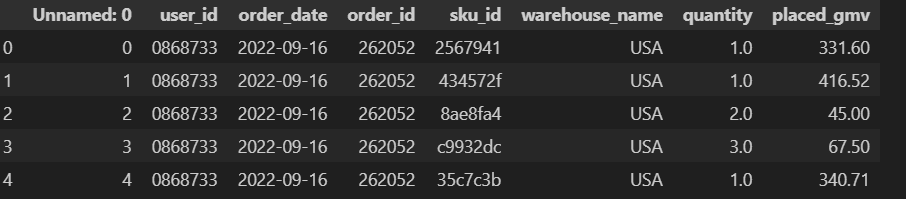
\includegraphics[width=1\columnwidth]{images/data_overview.png}
            \end{center}
            \answer{
                As clearly seen in the image, the dataset contains the following columns:
                \begin{itemize}
                    \item \texttt{Order\_ID}: Unique identifier for each order.
                    \item \texttt{User\_ID}: Unique identifier for each user.
                    \item \texttt{Order\_Date}: Date of the order.
                    \item \texttt{SKU\_ID}: Unique identifier for each product.
                    \item \texttt{Quantity}: Number of items purchased.
                    \item \texttt{Placed\_GMV}: Gross merchandise value (GMV) of the order.
            }
        }
        \item Inspect data for missing values, duplicates, and correct data types.{
            - Their are no missing values and duplicates in the dataset.\\
            \begin{center}
                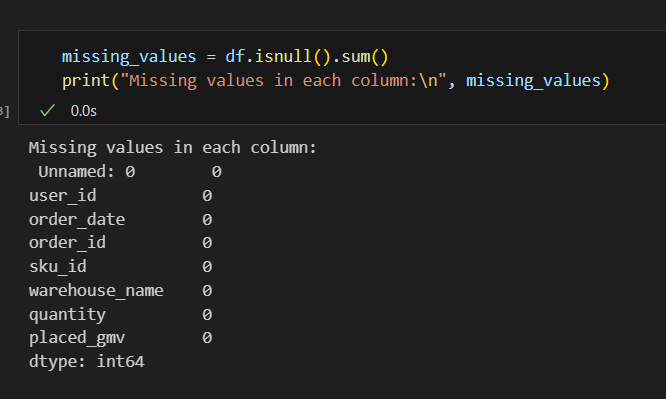
\includegraphics[width=1\columnwidth]{images/missing_values.png}
            \end{center}
        }
    \end{itemize}
    
    \subsection{Statistical Summary}
    \begin{center}
        \color{green}\rule{1\linewidth}{0.7mm}
    \end{center}
    \begin{center}
        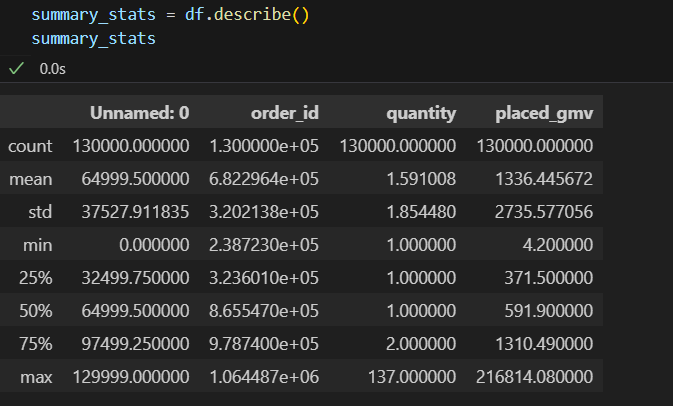
\includegraphics[width=1\columnwidth]{images/data-summary.png}
    \end{center}
    \answer{
       One thing we can observe from summary is that Quantity and Placed GMV are skewed and have outliers.\\
       As 75 percentile is 2 and 50 percentile is 1 for Quantity and 75 percentile is 1310.49 and 50 percentile is 591.90\\
        for Placed GMV.\\
       Whereas their Max values are 137 and 216814 which is much higher than 75 percentile.\\
    }
    
    \subsection{Date Formatting}
    \begin{center}
        \color{green}\rule{1\linewidth}{0.7mm}
    \end{center}
    This step is essential because the date column is in string format. We need to convert it to a datetime format for further analysis.{
        \begin{center}
            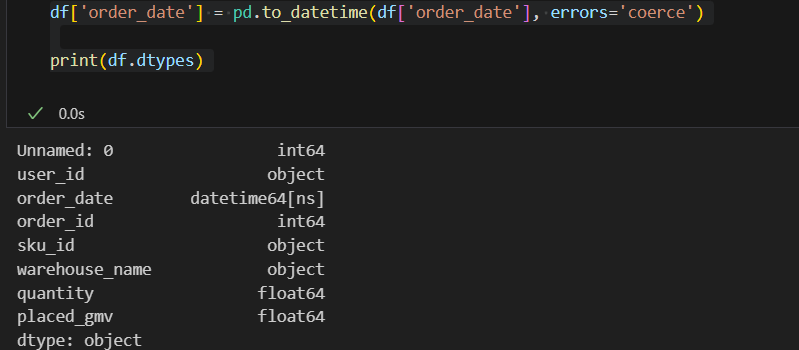
\includegraphics[width=1\columnwidth]{images/datatype.png}
        \end{center}
    }



\section{Customer Behavior Analysis}
    \subsection{Customer Purchase Frequency}
    Let's look at the distribution of frequency by which customers are placing orders .{
        \begin{center}
            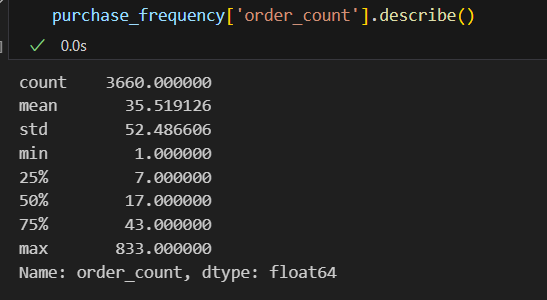
\includegraphics[width=1\columnwidth]{images/order-count.png}
        \end{center}
        \begin{tcolorbox}[colback=lightRed!5!white,colframe=lightRed!75!black,title=Insights]
            \textbf{Insights:}
            \begin{itemize}
                \item More than 50\% of customers have placed orders less than 17 times which is almost half than means\\.
                meaning few people are buying a lot.
                \item And 75\% of customers have placed orders less than 43 times.
                \item Just \textbf{293 people} out of 130000 have placed orders more than 100 times.
            \end{itemize}
        \end{tcolorbox}
    }
    \subsection{Top Customers}
    \begin{itemize}
        \item Based on Order frequency, I am identifying the top customers.{
            \begin{center}
                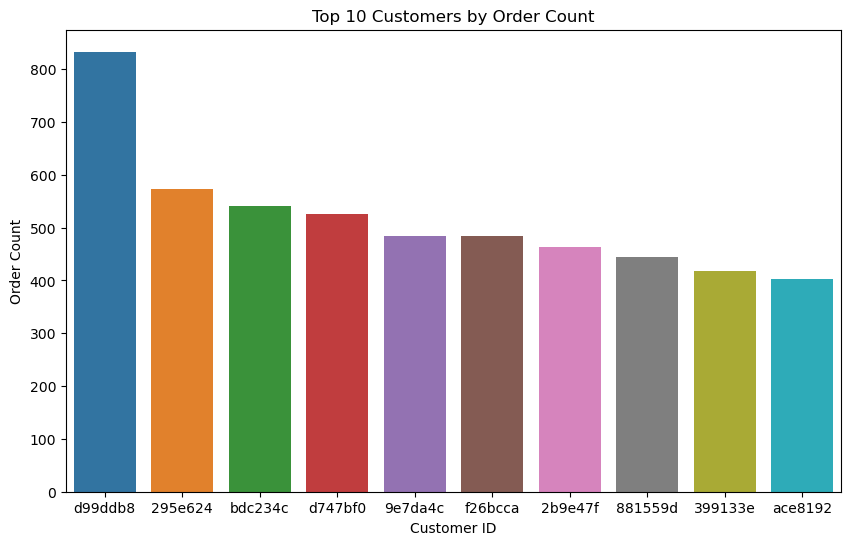
\includegraphics[width=1\columnwidth]{images/customer_purchase_frequency.png}
            \end{center}
        }
        
        
        \item Based on GMV, I am identifying the top customers.{
            \begin{center}
                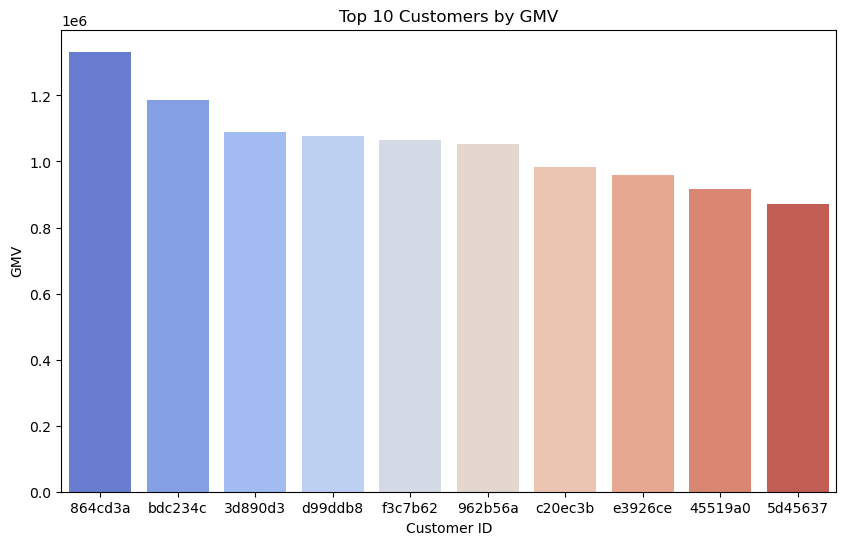
\includegraphics[width=1\columnwidth]{images/top_customers_by_gm.png}
            \end{center}
        }
    \end{itemize}
    
    \subsection{RFM Analysis}
    RFM analysis is a powerful way to segment customers based on their behavior.\\
\begin{itemize}
    \item Recency: When the customer last made a purchase.{
        Here i am calculating the recency of the customers.\\
        \begin{center}
            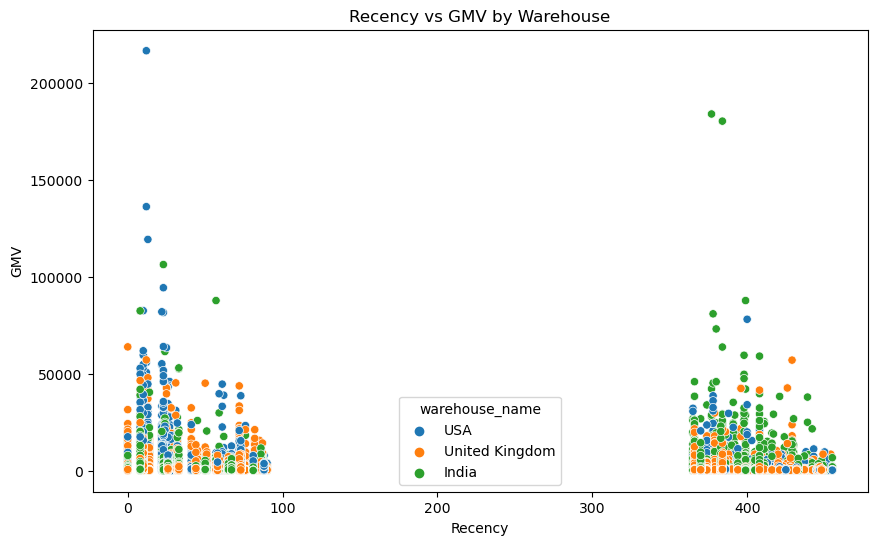
\includegraphics[width=1\columnwidth]{images/recency.png}
        \end{center}
        % use diff color for tcbox everytime
        \begin{tcolorbox}[colback=lightPink!5!white,colframe=lightPink!75!black,title=Insights]
            From the above graph, There are two types of custumers:-
            \begin{itemize}
                \item One who are frequent buyers and have bought recently less than 100 days.
                \item One who are seasonal buyers and have come to buy only after a year.
            \end{itemize}
        \end{tcolorbox}
    }
    \item Frequency: How often the customer made purchases.{
        Here i am calculating the how frequent customers have come to place orders.\\
        \begin{center}
            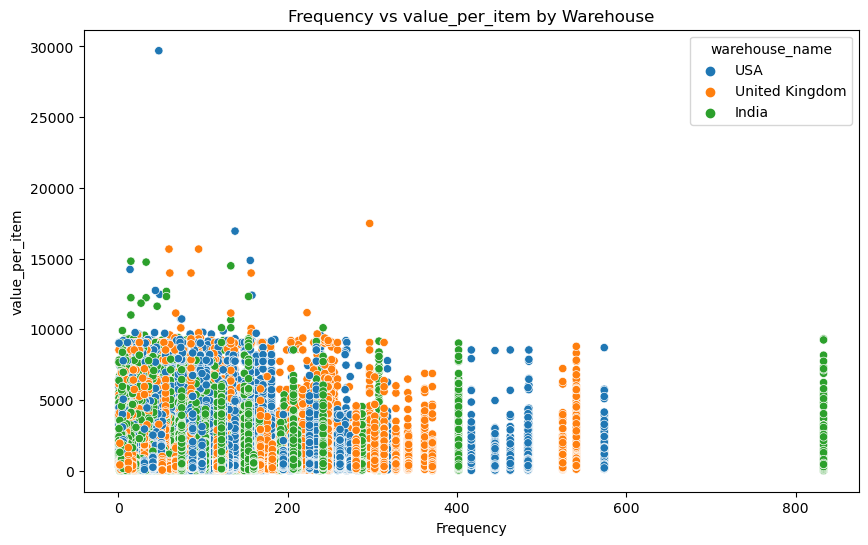
\includegraphics[width=1\columnwidth]{images/Freq_value.png}
        \end{center}
        \begin{tcolorbox}[colback=lightPink!5!white,colframe=lightPink!75!black,title=Insights]
            From the above graph, One observations is that low frequent buyers have more value\_per\_item than high frequent buyers.
        \end{tcolorbox}
    }
    \item Monetary: How much money the customer has spent.{
        Here i am calculating the how much money customers have spent.\\
        \begin{center}
            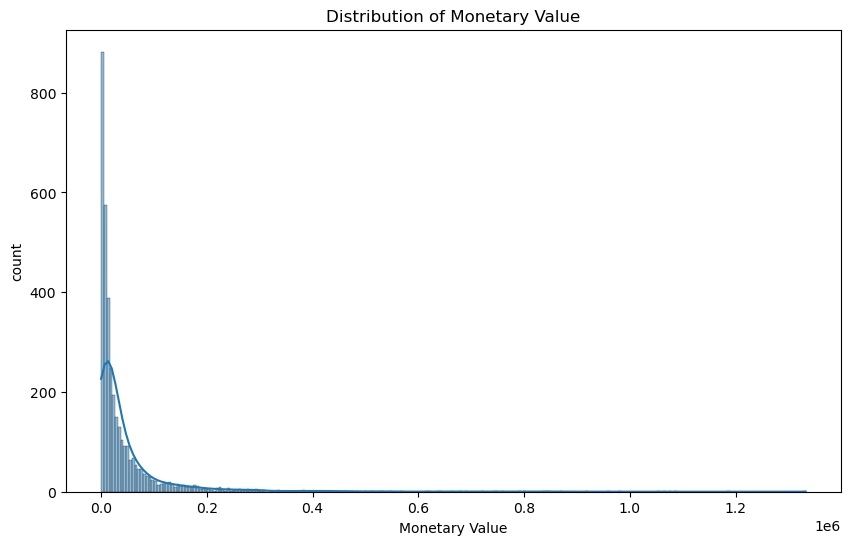
\includegraphics[width=1\columnwidth]{images/dist-mo.png}
        \end{center}
        \begin{tcolorbox}[colback=Pink!5!white,colframe=Pink!75!black,title=Insights]
           Majority of the people have spend less than 0.2 * 10^6.\\
        \end{tcolorbox}
    }
\end{itemize}

Now let's see the relationship between recency, frequency, and monetary values.{
    \begin{center}
        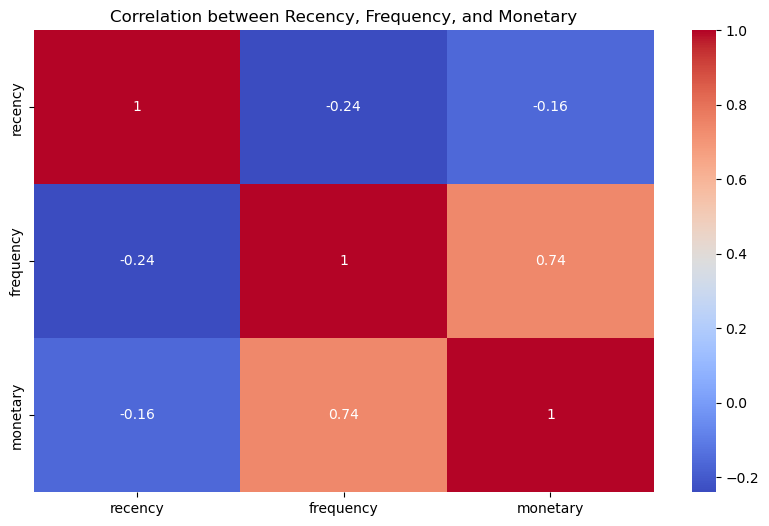
\includegraphics[width=1\columnwidth]{images/rfm.png}
    \end{center}
    \begin{tcolorbox}[colback=backgroundColor, colframe=accentColor2, title=Insights, fonttitle=\bfseries]
        \begin{itemize}
           \item From the above graph, we can see that there is a positive correlation between frequency and monetary value.\\
           \item But there is a negative correlation between recency and frequency and monetary value.\\
        \end{itemize}
       \end{tcolorbox}
}

\large
Score based on all three recency, frequency, and monetary values.\\
\begin{center}
    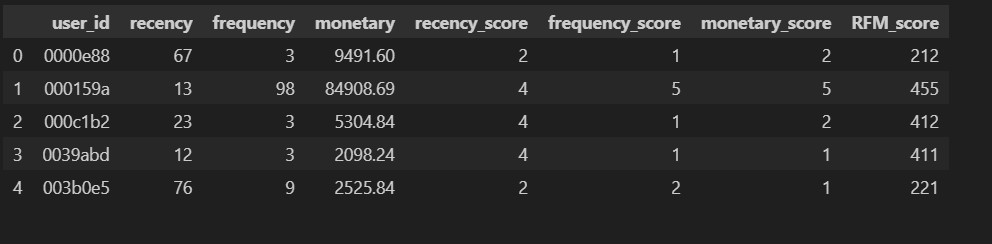
\includegraphics[width=1\columnwidth]{images/rfm-score.png}
\end{center}

\answer{
    Based on this score, i segmented customers into different categories such as:
    \begin{itemize}
        \item \textbf{Champions:} Customers with high recency, frequency, and monetary scores (R = 4-5, F = 4-5, M = 4-5).{

        }
        \item \textbf{Loyal Customers:}  Customers with high frequency and monetary scores but may have slightly lower recency (R = 3-5, F = 4-5, M = 4-5).
        \item \textbf{Potential Loyalists:} Customers with high recency and frequency but lower monetary value (R = 4-5, F = 3-5, M = 2-3).
        \item \textbf{New Customers:} High recency.
        \item \textbf{At Risk:} Low recency, frequency, and monetary value.
        \item \textbf{Lost:} Low recency, frequency, and monetary value.
    \end{itemize}
}

    
    
    \subsection{Customer Retention and Churn}
    \begin{itemize}
        \item Analyze customer retention rates and identify potential churn risks.
    \end{itemize}

\section{Sales Trends Analysis}
    \subsection{Time-based Trends}
    \begin{itemize}
        \item Analyze daily, weekly, and monthly sales trends.
    \end{itemize}
    
    \subsection{Peak Sales Periods}
    \begin{itemize}
        \item Identify peak sales periods and any seasonality trends.
    \end{itemize}
    
    \subsection{Year-over-Year Growth}
    \begin{itemize}
        \item Calculate year-over-year growth in sales.
    \end{itemize}
    
    \subsection{Average Order Value (AOV)}
    \begin{itemize}
        \item Analyze trends in average order value over time.
    \end{itemize}

\section{SKU Performance Analysis}
    \subsection{Top-Selling SKUs}
    \begin{itemize}
        \item Identify the top-selling SKUs based on quantity sold and GMV.
    \end{itemize}
    
    \subsection{SKU Diversity}
    \begin{itemize}
        \item Analyze the diversity of SKUs in customer orders.
    \end{itemize}
    
    \subsection{ABC Analysis}
    \begin{itemize}
        \item Perform ABC analysis to categorize SKUs based on sales contribution.
    \end{itemize}
    
    \subsection{Purchase Patterns}
    \begin{itemize}
        \item Examine SKU purchase patterns and correlations between items.
    \end{itemize}

\section{Order Analysis}
    \subsection{Order Sizes}
    \begin{itemize}
        \item Analyze the number of items per order.
    \end{itemize}
    
    \subsection{Relationship Between Order Size and GMV}
    \begin{itemize}
        \item Examine the relationship between order size and GMV.
    \end{itemize}
    
    \subsection{Multi-item Orders}
    \begin{itemize}
        \item Identify patterns in orders containing multiple items.
    \end{itemize}

\section{Cohort Analysis}
    \subsection{Customer Cohorts}
    \begin{itemize}
        \item Create cohorts based on the first purchase date of customers.
    \end{itemize}
    
    \subsection{Cohort Retention}
    \begin{itemize}
        \item Analyze retention rates and purchasing behavior over time for each cohort.
    \end{itemize}

\section{Geographic Analysis}
    \begin{itemize}
        \item Analyze sales distribution across different geographic regions.
        \item Identify high-performing and underperforming areas.
    \end{itemize}

\section{Time-based Analysis}
    \subsection{Order Patterns by Day and Time}
    \begin{itemize}
        \item Analyze patterns in order timing by day of the week and time of day.
    \end{itemize}
    
    \subsection{Promotion Opportunities}
    \begin{itemize}
        \item Identify potential opportunities for targeted promotions based on time-based analysis.
    \end{itemize}

\section{Customer Lifetime Value (CLV) Analysis}
    \subsection{CLV Calculation}
    \begin{itemize}
        \item Calculate customer lifetime value (CLV) for various customer segments.
    \end{itemize}
    
    \subsection{CLV Influencing Factors}
    \begin{itemize}
        \item Identify factors that influence CLV.
    \end{itemize}

\section{Basket Analysis}
    \subsection{Market Basket Analysis}
    \begin{itemize}
        \item Perform market basket analysis to identify frequently co-purchased items.
    \end{itemize}
    
    \subsection{Product Recommendations}
    \begin{itemize}
        \item Generate product recommendations based on customer purchase patterns.
    \end{itemize}

\section{Price Sensitivity Analysis}
    \subsection{Price vs. Demand}
    \begin{itemize}
        \item Analyze the relationship between price changes and demand for different SKUs.
    \end{itemize}
    
    \subsection{Price Optimization Opportunities}
    \begin{itemize}
        \item Identify opportunities for optimizing pricing strategies.
    \end{itemize}

\section{Visualization and Reporting}
    \begin{itemize}
        \item Create informative visualizations to present key insights from the data analysis.
        \item Prepare a comprehensive report summarizing findings and recommendations.
    \end{itemize}

\section{Advanced Analytics (Optional)}
    \subsection{Predictive Modeling}
    \begin{itemize}
        \item Develop predictive models for future sales and customer behavior.
    \end{itemize}
    
    \subsection{Customer Segmentation via Clustering}
    \begin{itemize}
        \item Perform clustering analysis to identify distinct customer segments.
    \end{itemize}

\section{Action Plan and Recommendations}
    \begin{itemize}
        \item Based on the insights, develop actionable recommendations to improve business performance.
    \end{itemize}

\end{document}



\end{document}